\chapter{Обучение и валидация модели}
\label{ch:training}

Здесь описана постановка обучения (функция потерь на обучающей выборке), метрики на отложенных данных, протокол разбиения по играм и краткое сравнение сохранённых прогонов~\cite{nikolenko2018}. Обозначения согласованы с главой~\ref{ch:theory}: $x$ --- входной текстовый признак, $y$ --- целевой вектор музыки, $\hat y$ --- предсказание модели.

\section{Постановка обучения}

Модель с параметрами $\theta$ задаёт отображение $f_\theta$, которое по входу $x_i$ выдаёт предсказание $\hat y_i = f_\theta(x_i)$. Обучение --- подбор $\theta$ по множеству примеров $\{(x_i, y_i)\}_{i=1}^n$, где пары уже собраны по процедуре главы~\ref{ch:dataset}. В качестве основной функции потерь используется средний квадрат отклонения по всем координатам и всем строкам обучения:
\begin{equation}
\mathcal{L}_{\mathrm{MSE}}(\theta) = \frac{1}{n d_y} \sum_{i=1}^n \sum_{k=1}^{d_y} \bigl( y_{ik} - f_\theta(x_i)_k \bigr)^2 .
\label{eq:mse-ch3}
\end{equation}
Такой выбор типичен для задачи восстановления вещественного вектора: он штрафует большие ошибки сильнее, чем малые, и гладкий по параметрам для методов стохастического градиента~\cite{nikolenko2018}. Дополнительно в коде могут использоваться отложение части строк игры для контроля переобучения, обрезка обучения по стагнации на валидации (\texttt{patience}), нормализация входов или целей --- конкретные значения указаны в \path{config.json} каждого прогона~\appa{5}.

\section{Метрики регрессии на тесте}

После обучения качество проверяют на строках, которые модель не использовала для подбора $\theta$. Ниже --- величины, которые сохраняются в \texttt{metrics.json}~\appa{5}.

\textbf{Средняя абсолютная ошибка и корень из среднего квадрата ошибки.} Для одной строки с истинным $y$ и предсказанием $\hat y$ задаются
\[
\mathrm{MAE}(y, \hat y) = \frac{1}{d_y} \sum_{k=1}^{d_y} |y_k - \hat y_k|, \qquad
\mathrm{RMSE}(y, \hat y) = \sqrt{\frac{1}{d_y} \sum_{k=1}^{d_y} (y_k - \hat y_k)^2}.
\]
Усреднение по всем тестовым строкам даёт поля \texttt{mae\_macro} и \texttt{rmse\_macro}: каждая координата вектора музыки входит с одинаковым весом. Интерпретация простая --- ``в среднем насколько единиц признака мы ошибаемся'', но разные координаты имеют разный масштаб в данных, поэтому без диагностики по столбцам это только общий индикатор.

\textbf{Косинус между векторами одной строки.} Иногда интересно, насколько предсказание ``сонаправлено'' с истиной в том же многомерном пространстве, без привязки к абсолютным масштабам координат:
\[
\cos(y, \hat y) = \frac{y^\top \hat y}{\|y\|\,\|\hat y\|}.
\]
По всем тестовым строкам усредняют --- поле \texttt{row\_cosine\_mean}. Большое значение не гарантирует малую MAE и не означает автоматически правильный выбор номера трека при ранжировании кандидатов.

\textbf{Линейная согласованность по столбцам.} Для каждого номера координаты $k$ считают выборочную корреляцию между истинными значениями этой координаты на тесте и предсказанными. Усреднение по столбцам даёт \path{column_pearson_mean} --- грубый индикатор того, воспроизводит ли модель хотя бы форму зависимости отдельных признаков.

\textbf{Коэффициенты $R^2$.} В логах также есть \texttt{r2\_macro} и \texttt{r2\_pooled}. На отложенных играх часть столбцов может иметь малую изменчивость, из-за чего показатель по столбцу становится неинформативным или численно неустойчивым; для выводов в данной работе опираются прежде всего на MAE, RMSE, средний косинус строки и метрику подстановки трека из следующего раздела.

\section{Метрика подстановки трека в списке кандидатов}
\label{sec:hit-at-p}

Отдельно от ошибки регрессии рассматривается задача, близкая к интерфейсу~\cite{nikolenko2018}: для тестовой строки данной игры известен истинный идентификатор трека и множество всех треков этой игры из каталога (глава~\ref{ch:dataset}). По предсказанному $\hat y$ каждый кандидатный трек со своим вектором $y^{(\mathrm{c})}$ получает оценку ``насколько он подходит'' --- например, больший косинус между $\hat y$ и $y^{(\mathrm{c})}$, или меньшую ошибку RMSE/MAE между этими векторами. Затем кандидаты сортируются; берётся верхняя доля $p$\% от размера пула $N$, то есть $t = \lceil pN/100\rceil$ лучших. Если истинный трек попадает в этот топ, считается попадание (hit). Доля таких случаев по всему тесту записывается в поля наподобие \texttt{retrieval\_cosine\_hit\_rate} для косинусного ранжирования и аналогично для RMSE и MAE.

Если упорядочить кандидатов случайно, доля попаданий была бы близка к $t/N$, то есть примерно к $p/100$ при больших $N$. Для основной серии экспериментов использовалось $p = 35$\%, то есть ориентир случайного уровня около $0{,}35$. Любая модель, дающая заметно больше, извлекает из текста хоть частично полезную информацию для сужения списка треков --- но до значений близких к единице сохранённые прогоны пока далеки.

\section{Разбиение выборки: обучение, валидация и тест}

Поддерживаются два режима аргумента \texttt{-{}-split}:

\begin{itemize}
	\item \texttt{within\_game} --- отложенная доля строк берётся внутри каждой игры; это проверка аппроксимации при уже знакомых играх;
	\item \texttt{leave\_games\_out} --- часть игр целиком исключается из обучения и используется для валидации и теста; учитываются только строки из оставшихся игр.
\end{itemize}

Для таблицы и рисунка ниже использован режим \texttt{leave\_games\_out}: число отложенных игр задаётся параметром \texttt{-{}-test-games} (в сохранённых прогонах обычно три игры), конкретный набор игр фиксируется генератором случайных чисел с семенем \texttt{held\_out\_games\_seed} (в основной серии значение $17$) --- стандартный приём оценки обобщения~\cite{nikolenko2018}. Так проверяется перенос на ``новый'' контент: модель не видела тестовую игру при подборе весов.

Внутри игр, отнесённых к обучению, выделяется доля строк для валидации (\texttt{-{}-val-fraction}, обычно $0{,}1$), при этом режим \texttt{-{}-val-split tail} берёт последовательный хвост по времени появления строк внутри игры --- чтобы не смешивать прошлое и будущее произвольным перемешиванием внутри одной истории. По валидации отслеживают улучшение функции потерь и останавливают обучение при отсутствии прогресса (параметры \texttt{patience} - число эпох без прогресса для остановки обучения). Цифры на валидации часто заметно лучше, чем на полностью новых играх (в валидации исползьовался режим `sqlit tail`, а в тестовой выборке всегда выделялись игры. Это говорит о том, что модели очень хорошо подстраиваются под игры в обучаемой выборке, но хуже в обобщении); для выводов о приложении предпочтителен именно тест с отложенными играми.

\section{Воспроизводимость и артефакты}

\begin{sloppypar}
Глобальный параметр \texttt{seed} инициализации и семя разбиения игр сохраняются в~\path{config.json}~\appa{5}. Файл \path{manifest.jsonl}~\appa{3} связывает логическое имя прогона, командную строку и каталог вывода в дереве сохранённых прогонов~\appa{5}. В каждой папке прогона есть \path{metrics.json}, опционально \path{per_column_metrics.csv} и журнал \path{stdout.log}~\appa{5}. Единый каталог артефактов доступен как \path{artifacts/runs/} (ссылка на то же дерево, см.~\appa{5}).
\end{sloppypar}

\section{Результаты}

Под этим заголовком собран разбор сохранённых численных итогов и материала логов: от протокола, по которому снята таблица, до качественных выводов о том, как ведёт себя ошибка по эпохам и где виден разрыв между валидацией на знакомых играх и тестом на отложенных играх. Базовые определения метрик и режим разбиения выборки задаются разделами выше в текущей главе; здесь они используются как уже введённые обозначения.

\subsection{Протокол, воспроизводимость и сводная таблица}

Ниже интерпретируются прогоны при единых условиях: \texttt{leave\_games\_out}, три отложенные игры, семя \texttt{held\_out\_games\_seed}=17, доля топа $p=35$\% для ранжирования кандидатов (раздел~\ref{sec:hit-at-p}). Из сводной выборки для таблицы исключены диагностический прогон с другим процентом топа ($p=50$), записи без собственной папки результатов на диске и короткие локальные серии с префиксом \texttt{local\_}; отдельный прогон GRU при иных параметрах топа или семени игр в таблицу не включался. Такие ограничения совпадают с правилами скриптов автоматической агрегации~\appa{6} в репозитории~\appa{1}; технические имена файлов конфигурации и метрик в дереве~\appa{5} уже описаны разделом о воспроизводимости.

Таблица~\ref{tab:main-runs} содержит тестовый MAE, среднее столбцов корреляции Пирсона $\overline{\rho}$, несколько версий retrieval-hit (cos, RMSE, MAE в смысле раздела о метрике подстановки) и число фактических эпох до остановки по валидации. Хотелось бы иметь столбцы, однозначно отражающие интерес конечного пользователя, но они складываются из регрессии по $320$-мерному описанию треков и упрощающего ранжирования только внутри одной игры: потому здесь имеет смысл читать и MAE/\,$\overline{\rho}$, и \textit{cos hit} сообща, без выбора единственного ``главного'' числа.

\begin{table}[H]
\centering
\caption{Тестовые метрики сохранённых прогонов (основной протокол).}
\label{tab:main-runs}
\footnotesize
\resizebox{\textwidth}{!}{% auto-generated by scripts/aggregate_run_metrics.py (aggregate_rubert_run_metrics.py)
% do not edit by hand; re-run the script after new runs
\begin{tabular}{|l|l|r|r|r|r|r|r|}
\hline
прогон & семейство & MAE & $\overline{\rho}$ & cos hit & RMSE hit & MAE hit & эп. \\
\hline
\texttt{run\_019\_autoreg\_light\_budget} & mlp\_autoreg\_lags & 0.456 & 0.226 & 0.609 & 0.565 & 0.515 & 32 \\
\texttt{run\_002\_lstm} & lstm & 0.473 & 0.122 & 0.601 & 0.582 & 0.608 & 43 \\
\texttt{run\_008\_mlp\_hugelags} & mlp\_lags & 0.504 & 0.058 & 0.577 & 0.473 & 0.472 & 41 \\
\texttt{run\_017\_tcn\_lag8\_softer} & tcn & 0.488 & 0.176 & 0.574 & 0.536 & 0.555 & 63 \\
\texttt{run\_018\_tf\_small\_win} & transformer\_window & 0.505 & 0.023 & 0.573 & 0.514 & 0.546 & 110 \\
\texttt{run\_001\_mlp\_autoreg\_lags} & mlp\_autoreg\_lags & 0.489 & 0.320 & 0.571 & 0.585 & 0.538 & 44 \\
\texttt{run\_003\_tcn} & tcn & 0.497 & 0.171 & 0.556 & 0.505 & 0.545 & 85 \\
\texttt{run\_012\_lstm\_like002\_seed39} & lstm & 0.455 & 0.203 & 0.555 & 0.582 & 0.560 & 45 \\
\texttt{run\_006\_tcn} & tcn & 0.544 & 0.183 & 0.555 & 0.582 & 0.601 & 37 \\
\texttt{run\_005\_lstm} & lstm & 0.672 & 0.172 & 0.555 & 0.582 & 0.513 & 21 \\
\texttt{run\_014\_lstm\_lag6\_compact} & lstm & 0.451 & 0.155 & 0.555 & 0.582 & 0.608 & 35 \\
\texttt{run\_013\_lstm\_like002\_seed41} & lstm & 0.480 & 0.145 & 0.555 & 0.549 & 0.558 & 18 \\
\texttt{run\_009\_lstm} & lstm & 0.444 & 0.095 & 0.555 & 0.582 & 0.559 & 59 \\
\texttt{run\_001\_mlp\_biglags} & mlp\_lags & 0.495 & 0.110 & 0.540 & 0.435 & 0.437 & 90 \\
\texttt{run\_007\_transformer\_window} & transformer\_window & 0.531 & -0.001 & 0.540 & 0.536 & 0.550 & 84 \\
\texttt{run\_010\_tcn} & tcn & 0.603 & 0.150 & 0.486 & 0.640 & 0.555 & 33 \\
\texttt{run\_004\_transformer\_window} & transformer\_window & 0.545 & 0.001 & 0.437 & 0.362 & 0.377 & 100 \\
\texttt{run\_011\_transformer\_window} & transformer\_window & 0.553 & 0.004 & 0.436 & 0.294 & 0.371 & 138 \\
\hline
\end{tabular}
}
\end{table}

\subsection{Короткие обозначения прогонов в тексте}

В первой колонке таблицы приводятся технические имена каталогов; соответствие результатов журналам и файлам конфигурации задаётся структурой хранения прогонов~\appa{5}. Каталог сохранений в репозитории обозначен как \path{rubert_runs/}. Чтобы дальше не повторять длинные строки имён каталогов, в тексте используются читаемые обозначения. До поясняющего списка ниже они задают только укрупнённую ссылку ``к строке таблицы и семейству архитектуры'', а не заменяют точное имя при сопоставлении с файлом результатов:

\begin{itemize}
	\item \textbf{LSTM} --- сохранённый прогон LSTM с несколькими лагами текстового эмбеддинга, из основной серии с отложенными играми и топом $35$\%; по числу cosine-hit это близкий конкурент лидирующей авторегрессионной конфигурации второй строки таблицы. Полный комплект конфигурации и протоколов, итоговые \texttt{metrics.json}, а также текст \texttt{stdout.log} доступны как отдельный электронный архив~\appa{8}. Две буквы <<LSTM>> без номера далее обозначают семейство в целом, а связка <<LSTM>> привязана именно к этому сохранённому прогону.
	\item \textbf{AR} или \textbf{Авторегрессия} --- облегчённая авторегрессионная конфигурация с лучшим в таблице \textit{cos hit} порядком $0{,}609$ (верхняя строка); разумеется, имя её каталога читают прямо из первого столбца той же таблицы.
	\item Прочие краткие подписи вроде \textbf{TCN}, \textbf{Transformer~(тяжёлое окно)} и~\textbf{MLP-большие лаги} при первом упоминании отправляют к колонке <<семейство>> таблицы~\ref{tab:main-runs} и к конкретной строке, если из контекста и так ясно, какая конфигурация имеется в виду; при малейшем сомнении остаётся прямое чтение идентификатора прогона.
\end{itemize}

Такой способ упрощает чтение, не заменяя строго фиксирующих технических названий там, где важно одно к одному сопоставление с файлом результатов~\appa{5}.

\subsection{Интерпретация качества регрессии и ранжирования}

Среднее MAE около $0{,}45$--$0{,}50$ у строк верхней половины таблицы говорит об умеренной суммарной ошибке координат, но каждая координата отражает свой аспект аудиопризнака и тега, масштаб и изменчивость которых между играми сильнее разъезжаются, чем ожидалось бы по одной средней регрессии. Это поддерживают умеренные значения среднего столбцового Пирсона $\overline{\rho}$ на новых играх: они чаще оказываются порядка $0{,}1$--$0{,}2$ у большинства устойчивых архитектур, нежели <<почти идеальной линейной копией>> столбца за столбцом. Отдельно отмечены трансформеры с высокими вычислительными затратами~\cite{vaswani2017}: здесь уже встречаются значения $\overline{\rho}$, близкие к нулю, хотя параметризация намного сложнее линейного уровня.

Так видно, что текст отчётливо сдвигает распределение кандидатов от полной случайности (ориентир $p/100\approx 0{,}35$ при топе доли $p=35$\%, раздел~\ref{sec:hit-at-p}), но до уровня ``почти всегда нашли нужный трек'' по сохранённым данным типичное cosine-hit всё ещё далеко, и упорядочивание без второго мнения человека использовать рискованно. Совпадающее после округления значение cosine-hit у нескольких соседних LSTM в таблице отражает дискретность метрики на конечном тестовом множестве строк, а не обязательное совпадение качества между различными сохранёнными каталогами.

Трансформер с большим окном памяти в этой же серии оказывается заметно слабее по cosine-hit, чем AR и LSTM, и подчёркивает, что добавление параметров и логарифма вычислительной тяжести автоматически не выводит задачу MSE~\eqref{eq:mse-ch3} к лучшему упорядочиванию кандидатов в пространстве музыкальных векторов.

\subsection{Эксперимент по фильтрации ``активных'' столбцов музыки на тесте}

Дополнительно рассматривалась фильтрация столбцов вектора $y$ на этапе тестирования: в агрегаты ошибки и retrieval попадали только координаты, которые по эмпирическому активному разбросу не выродились в почти постоянную величину. На всех прогонах, для которых эта версия счёта применялась, наблюдалось падение cosine-hit порядком с около $0{,}6$ до около $0{,}4$ относительно измерений без фильтра. Разбор причин смешения масштабов ранжирования при этом не был зафиксирован в сохранённых \texttt{metrics.json}, поскольку соответствующие полные дампы утрачиваются между машинами; отсюда в тексте только запомненный качественный эффект. Для воспроизводимости стоило бы сохранять такие прогоны в отдельных каталогах \texttt{rubert\_runs} с записью режима счёта в \texttt{manifest.jsonl}.

\subsection{Кривые обучения: MSE и MAE для train и val по эпохам}

В \texttt{stdout.log} печатаются строки вида epoch: они содержат \texttt{train\_mse}, нормализованные MAE для train и val, показатель лучшей валидации и параметры счётчика patience. Таким образом, динамика минимизации MSE~\eqref{eq:mse-ch3} и сопряжённые MAE читаются прямо из журнала, не распаковывая тензорные дампы состояния оптимизации~\appa{5}.

На рисунке~\ref{fig:train-curves} шесть характерных прогонов из основной серии подписаны согласованно с читаемыми именами LSTM, AR и несколькими соседними конфигурациями; это же изображение демонстрирует, как выглядит одновременное сравнение семейства кривых на одном листе. Верхний подграфик --- train MSE; нижний --- нормы MAE, где более прозрачный пунктир обозначает train, более насыщенная сплошная --- val того же цвета. Для авторегрессионных скриптов в логах к полям добавляются суффиксы \texttt{\_seq}, но для глаза кривая остаётся той же по смыслу. Изображение сформировано скриптом \path{scripts/plot_training_stdout_curves.py}~\appa{9}, входом которого служит перечень выбранных каталогов \texttt{run\_*}.

\begin{figure}[H]
\centering
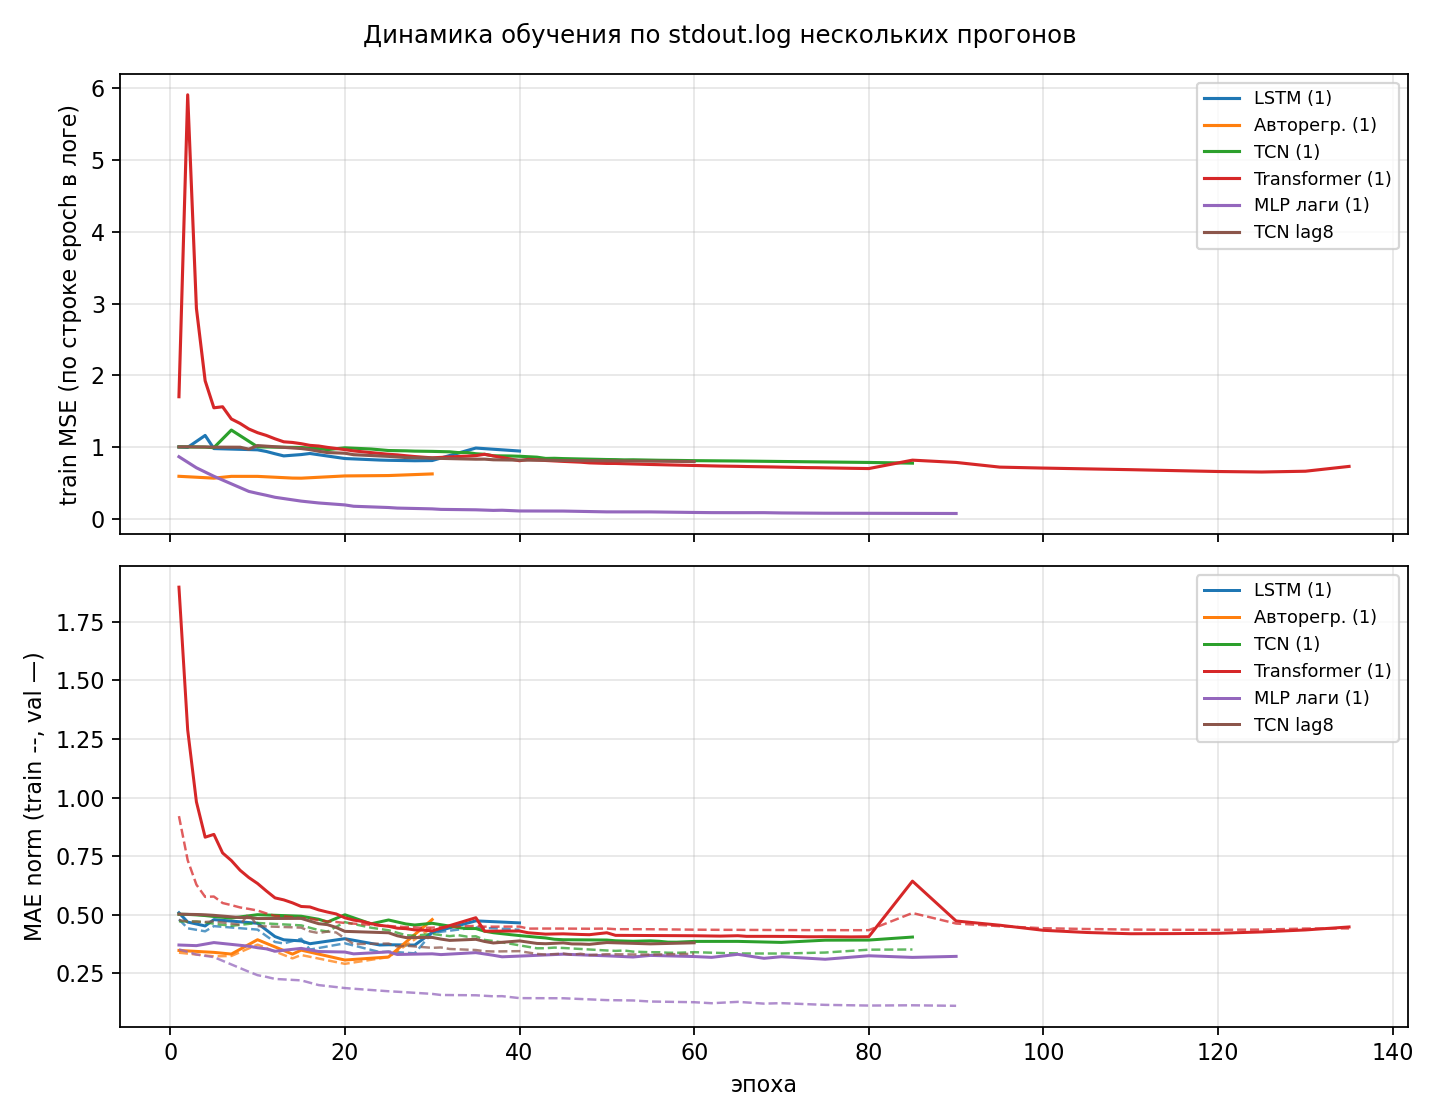
\includegraphics[width=0.95\textwidth]{images/training_stdout_mse_mae_curves.png}
\caption{По каждому выбранному прогону: сверху динамика train MSE; снизу нормализованный MAE (пунктир --- train, сплошная --- val). Короткая подпись в легенде соответствует читаемому имени архитектуры; полные имена каталогов см.~\protect\appa{5}, пример связки каталог\,--\,текста лога ---~\protect\appa{8}.}
\label{fig:train-curves}
\end{figure}

Совместное наблюдение train и val на одном экране удобно для поиска ситуации, когда ошибка по обучению продолжает падать без отражения во внимательной валидации: там срабатывает раннее прерывание по patience. Эти графики иллюстрируют, почему в разделах о протоколе подчёркивался различный вклад строк тестирования между валидацией и финальными играми, не участвовавшими в обучении.

\subsection{Столбчатая диаграмма cosine-hit для основной серии}

Столбчатая диаграмма (рисунок ниже) визуализирует сохранённые \textit{cos hit}; горизонтальная черта соответствует ориентиру случайного ранжирования при топе доли $p=35$\%, как в определении раздела~\ref{sec:hit-at-p}.

\begin{figure}[H]
\centering
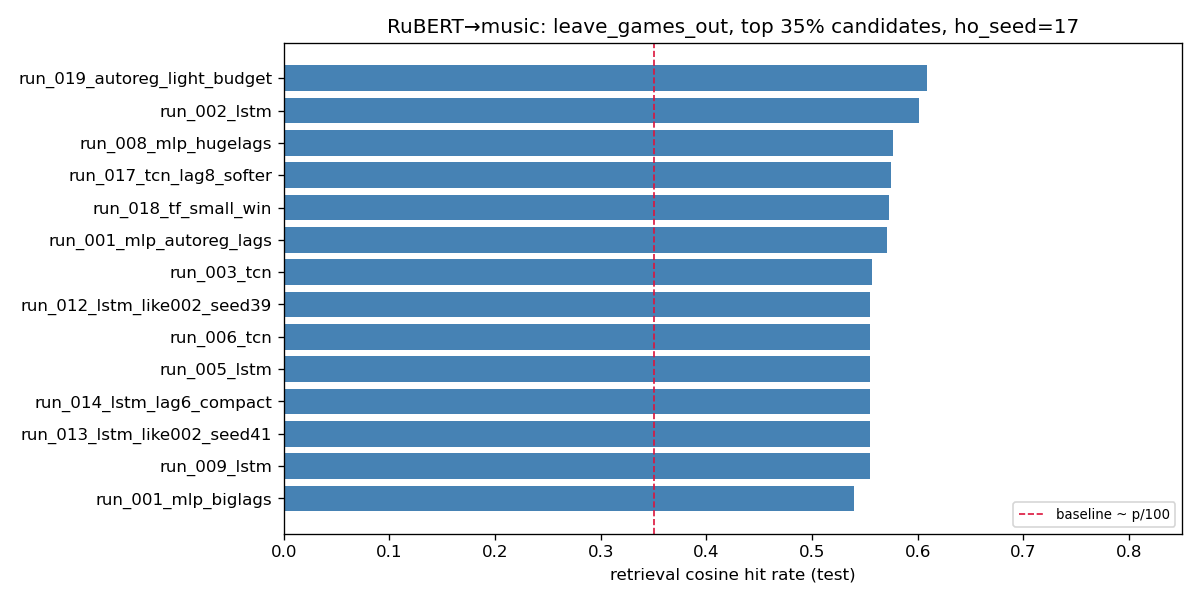
\includegraphics[width=\textwidth]{images/retrieval_cosine_hit_p35.png}
\caption{Доля попаданий истинного трека в топ $35$\% кандидатов при ранжировании по косинусу (\texttt{leave\_games\_out}, \texttt{held\_out\_games\_seed}=17).}
\label{fig:retrieval-bar}
\end{figure}

\subsection{Что имеет смысл сделать дальше и краткий вывод для приложения}

Практически ближайший шаг --- пропустить лучшие сохранённые веса через \emph{инференс} на типичной пользовательской машине и измерить задержку ответа: модель интересует только там, где она укладывается в темп чтения и не превращает сценарий Lyrata в загрузчик тяжёлых экспериментов.

Отдельно незаменим субъективный тест: свой реальный текст, свой любимый плейлист и ручное прогонывание нескольких сцен наблюдения после обучения. Числовая таблица и кривая ошибки уже показывают, что сигнал есть, но ощущается ли он комфортно при живом восприятии, без нескольких вечеров <<наощуп>> иногда просто не выясняется.

Дальнейшие общие технические задачи сохраняют линию, озвученную ранее: расширение датасета, функции потерь ближе к парному или списковому ранжированию, контроль утечки информации и документирование редких диагностических перезапусков через отдельные записи \texttt{manifest.jsonl}.

Для сценария приложения суммарный результат остаётся тем же даже после развёрнутой табличной статистики: при лучших числах истинная дорожка в среднем только чуть чаще оказывается внутри тридцати пятой доли упорядоченных кандидатов и редко когда обходится без участия человека при окончательном выборе. Модель уместнее трактовать как вспомогательное упорядочивание набора дорожек, а не источник окончательного решения.
